%% Two-page precis of the PhD thesis proposal
%% Knox, 2026.
%%
%% The copy that is attached to a first email. It has to stand alone on two
%% pages, and it is ordered as an argument a reader can follow without the
%% proposal: the question in plain words, and the idea in one sentence; the
%% figure, which is the statement aimed at, drawn where a landing footprint
%% is drawn; why the bound that is free is useless; what it ignores; the
%% theorem aimed at; the obstacle; what is open. Build with
%% `make proposal-precis`; `make proposal-dist` names the copy to attach.
%%
%% Three rules hold here, as in main.tex.
%%   The subject is hypersonic entry: any vehicle, any corridor. One flight
%%   appears, as the example the figure's trajectory is taken from, and it
%%   is named only there.
%%   Nothing is claimed as done. This is a proposal: no preliminary
%%   derivation, computation or check is reported, and the sets in the
%%   figure are an illustration, which the figure and its caption both say.
%%   No software is referred to or promised.
%%
%% It shares the preamble and the bibliography with main.tex, and nothing
%% else: no cross-reference reaches from here into the proposal, so the two
%% cannot fall out of step by a renumbering. What CAN fall out of step is
%% the wording of the target statement. Reread it when main.tex changes.
%%
%% The header carries no link. The proposal goes with the email, as an
%% attachment or on request; a link, when there is a place to host it,
%% belongs on the line under the date.

\documentclass[english,10pt]{extarticle}
\usepackage[T1]{fontenc}
\usepackage[utf8]{inputenc}
\usepackage{geometry}
\geometry{verbose,tmargin=1in,bmargin=1in,lmargin=1in,rmargin=1in}
\usepackage{float}
\usepackage{booktabs}
\usepackage{tabularx}
\usepackage{amsmath}
\usepackage{amsthm}
\usepackage{amssymb}
\usepackage{bm}
\usepackage{graphicx}
\usepackage{units}
\usepackage{enumitem}
\usepackage{microtype}          % typographic polish: char protrusion, expansion
\usepackage{xcolor}
\usepackage{comment}
\usepackage{tcolorbox}          % highlighted result boxes
\tcbuselibrary{skins,breakable}
\usepackage{fancyhdr}           % running header with the short title
\usepackage[textsize=footnotesize]{todonotes}   % margin \todo{} notes; width follows \marginparwidth
\usepackage{authblk}

\makeatletter

\numberwithin{equation}{section}
\numberwithin{figure}{section}
\numberwithin{table}{section}

% ---- Theorem environments ----
\@ifundefined{thm}{%
  \theoremstyle{plain}%
  \newtheorem{thm}{Theorem}[section]%
}{}
\@ifundefined{prop}{\newtheorem{prop}[thm]{Proposition}}{}
\@ifundefined{lem}{\newtheorem{lem}[thm]{Lemma}}{}
\@ifundefined{cor}{\newtheorem{cor}[thm]{Corollary}}{}
\@ifundefined{conj}{\newtheorem{conj}[thm]{Conjecture}}{}
\@ifundefined{defn}{%
  \theoremstyle{definition}%
  \newtheorem{defn}[thm]{Definition}%
}{}
\@ifundefined{assum}{%
  \theoremstyle{definition}%
  \newtheorem{assum}[thm]{Assumption}%
}{}
\@ifundefined{example}{\newtheorem{example}[thm]{Example}}{}
\@ifundefined{remark}{%
  \theoremstyle{remark}%
  \newtheorem{remark}[thm]{Remark}%
}{}

% ---- Convenient macros ----
\newcommand{\R}{\mathbb{R}}
\newcommand{\C}{\mathbb{C}}
\newcommand{\N}{\mathbb{N}}
\newcommand{\E}{\mathbb{E}}
\newcommand{\Prob}{\mathbb{P}}
\newcommand{\ip}[2]{\langle #1, #2 \rangle}
\newcommand{\norm}[1]{\left\| #1 \right\|}
\newcommand{\abs}[1]{\left| #1 \right|}
\newcommand{\T}{^{\mathsf{T}}}          % transpose
\newcommand{\dd}{\,\mathrm{d}}          % upright differential
\newcommand{\D}[2]{\frac{\mathrm{d}#1}{\mathrm{d}#2}}     % total derivative
\newcommand{\pd}[2]{\frac{\partial #1}{\partial #2}}      % partial derivative

% ---- Program-wide notation ----
\newcommand{\Rset}{\mathcal{R}}          % reachable set
\newcommand{\Mplus}{\mathcal{M}_+}       % cone of nonnegative Radon measures
\newcommand{\Xset}{\mathcal{X}}          % state constraint set
\newcommand{\Uset}{\mathcal{U}}          % control constraint set
\newcommand{\Lie}{\mathcal{L}}           % Lie derivative / generator
\newcommand{\modes}{\mathcal{Q}}         % mode alphabet (Paper 1, Section 2.2)
\newcommand{\guard}{\mathcal{S}}         % guard surface
\newcommand{\reset}{\mathcal{J}}         % reset map

% The Henrion-Korda dual pair is conventionally (v, w). Both letters are
% already body-frame velocity components in the state vector, and the
% certificate is a function OF that state, so the two would collide inside a
% single displayed equation. Capital Greek instead: distinct from latitude
% \phi and heading \psi, which are lowercase. Named here so the choice is
% changed in one place rather than hunted through the papers.
\newcommand{\cert}{\Phi}               % Liouville supersolution, cert(t,x)
\newcommand{\certT}{\Psi}              % terminal majorant, certT(x)

\makeatother

% ---- Highlighted-result box ----
\newtcolorbox{keybox}[1][]{colback=blue!4,colframe=blue!45!black,
  boxrule=0.6pt,arc=2pt,left=6pt,right=6pt,top=4pt,bottom=4pt,#1}

% ---- Development annotations ----
%  Three coloured boxes carrying the drafting ledger inside the source:
%    decide -- a choice made, recorded so it is not silently re-opened
%    gap    -- an obligation not yet discharged
%    idea   -- a line of argument worth keeping, not yet load-bearing
%  They are deliberately conspicuous. Set \draftnotesfalse below (or pass
%  \PassOptionsToPackage before \input{preamble}) to compile a submission
%  copy in which all three vanish, exactly as [disable]{todonotes} removes
%  the \todo list --- the boxes must not survive into a submitted draft,
%  and a single switch is the only reliable way to be sure of that.
\newif\ifdraftnotes
\draftnotestrue

\newtcolorbox{decide@box}[1][]{colback=orange!4,colframe=orange!45!black,
  boxrule=0.6pt,arc=2pt,left=6pt,right=6pt,top=4pt,bottom=4pt,#1}
\newtcolorbox{gap@box}[1][]{colback=red!4,colframe=red!50!black,
  boxrule=0.6pt,arc=2pt,left=6pt,right=6pt,top=4pt,bottom=4pt,#1}
\newtcolorbox{idea@box}[1][]{colback=green!4,colframe=green!35!black,
  boxrule=0.6pt,arc=2pt,left=6pt,right=6pt,top=4pt,bottom=4pt,#1}

\ifdraftnotes
  \newenvironment{decide}{\begin{decide@box}}{\end{decide@box}}
  \newenvironment{gap}{\begin{gap@box}}{\end{gap@box}}
  \newenvironment{idea}{\begin{idea@box}}{\end{idea@box}}
\else
  \excludecomment{decide}
  \excludecomment{gap}
  \excludecomment{idea}
\fi

% ---- Theorem-environment aliases ----
%  The drafts write \begin{assumption} and \begin{lemma} in full; the
%  counters above are declared as assum and lem. Alias rather than rename,
%  so neither spelling is a compile error and no draft has to be rewritten
%  to match a decision about abbreviation.
\makeatletter
\@ifundefined{assumption}{%
  \newenvironment{assumption}[1][]{\begin{assum}[#1]}{\end{assum}}}{}
\@ifundefined{lemma}{%
  \newenvironment{lemma}[1][]{\begin{lem}[#1]}{\end{lem}}}{}
\makeatother

\usepackage{babel}

% ---- Cross-references and links (load late: hyperref then cleveref) ----
\usepackage[hidelinks,colorlinks=true,
  linkcolor=blue!55!black,citecolor=blue!55!black,urlcolor=blue!55!black]{hyperref}

% ---- Bibliography ----
%  biblatex, not the plain BibTeX \bibliography. Loaded after hyperref and
%  before cleveref, which is the order the biblatex manual asks for.
%
%  style=numeric keeps the bare-number in-text appearance the papers have
%  always used. sorting=none orders the reference list by first citation,
%  which reads better than alphabetical in a proposal.
%
%  sortcites is the one non-obvious option. It sorts the keys WITHIN each
%  citation so the numeric style can collapse consecutive labels into a
%  range -- without it a five-key \parencite renders as five separate
%  brackets. Note this is NOT natbib's sort&compress, which biblatex does
%  not provide: the biblatex natbib compatibility layer (blx-natbib.def)
%  defines \citep and \citet but nothing for compression, and an unknown
%  package key only warns, so a wrong setting here fails silently.
%
%  maxcitenames=2 keeps a multi-key citation from printing every author;
%  maxbibnames=99 with giveninits stops the reference list collapsing long
%  author lists to "et al." in a way that would not match the full lists
%  written out in shared.bib (see emmert2021nrlmsis, hersbach2020era5).
%
%  The per-entry reading notes in the bibliography live in the biblatex
%  `annotation' field. They are the most valuable content in that file and are
%  deliberately NOT printed. Note that `annotation' is a DATA field, not an
%  option of \printbibliography -- passing annotation=false to \printbibliography
%  is an xkeyval error, not a way of suppressing it. Blanking the field's format
%  is the mechanism, and it is the right one: the notes survive in the .bib and
%  in the .bbl for the author's use, and never reach the page. This must come
%  AFTER the \usepackage line below, since \DeclareFieldFormat is defined there.
\usepackage[backend=biber,style=numeric,sorting=none,sortcites,
  maxbibnames=99,giveninits=true,maxcitenames=2]{biblatex}

% biblatex requires csquotes whenever babel is loaded, and warns without it
% ("'babel/polyglossia' detected but 'csquotes' missing"). It supplies the
% quote punctuation the bibliography macros expect. Not currently used by any
% entry, but the dependency is unconditional.
\usepackage{csquotes}

\DeclareFieldFormat{annotation}{}

% The thesis bibliography. \addbibresource must be issued in the preamble, and
% this preamble is \input from a directory one level below manuscript/, so the
% path is written relative to that directory, not to this file.
\addbibresource{../thesis.bib}

\usepackage[nameinlink,capitalise]{cleveref}

% ---- Running header: each paper calls \runninghead{Short Title} ----
\newcommand{\runninghead}[1]{%
  \pagestyle{fancy}%
  \fancyhf{}%
  \lhead{\small #1}%
  \rhead{\small\thepage}%
  \renewcommand{\headrulewidth}{0.3pt}%
}

\geometry{margin=0.8in}
\pagestyle{plain}
\hypersetup{
  pdftitle={Certified analytical bounds for hypersonic reachable sets: a two-page summary},
  pdfauthor={Ethan Knox},
  pdfsubject={Summary of a preliminary PhD research proposal},
}
\ExecuteBibliographyOptions{maxbibnames=3,doi=false,isbn=false,url=false}
\renewcommand*{\bibfont}{\footnotesize}
\setlength{\bibitemsep}{1pt}
\setlength{\parskip}{0pt}
% The preamble numbers figures within sections, and this copy has none.
\renewcommand{\thefigure}{\arabic{figure}}
% One figure, set here: its caption a size down, and no more air around it
% than separates two paragraphs of a section.
\makeatletter
\long\def\@makecaption#1#2{\vskip 4pt{\small #1: #2\par}}
\makeatother
\setlength{\intextsep}{7pt plus 2pt minus 1pt}

\newcommand{\head}[1]{\par\smallskip\noindent\textbf{#1}\enspace}

\begin{document}

\begin{center}
  {\Large\bfseries Certified analytical bounds for hypersonic reachable
  sets}\\[0.3em]
  {\itshape A two-page summary of a preliminary PhD research proposal}\\[0.5em]
  Ethan Knox\quad\textperiodcentered\quad Champaign, IL\quad
  \textperiodcentered\quad \today
\end{center}

\head{The question.}
A vehicle entering an atmosphere at hypersonic speed can be steered, within
limits, and neither the air nor its own aerodynamics is known better than
within tolerances. What can it be driven to? The states it can reach under
\emph{every} admissible control and every admissible model form its
reachable set, which a safety analysis has to enclose; a landing
footprint is its shadow on the ground. This proposal is about an
\emph{outer} bound on it that is proved and not
sampled, and that is a formula: explicit in the vehicle and the flight
corridor, to be evaluated again, not solved for again, when either changes.
The idea is that the thin atmosphere supplies one: in the limit a flight is
a slow motion punctuated by brief passes through dense air, and the bound
sought is the reachable set of that much smaller limit system, thickened by
an explicit margin. The vehicle is a parameter of the bound, not its
subject.

\begin{figure}[h]
  \centering
  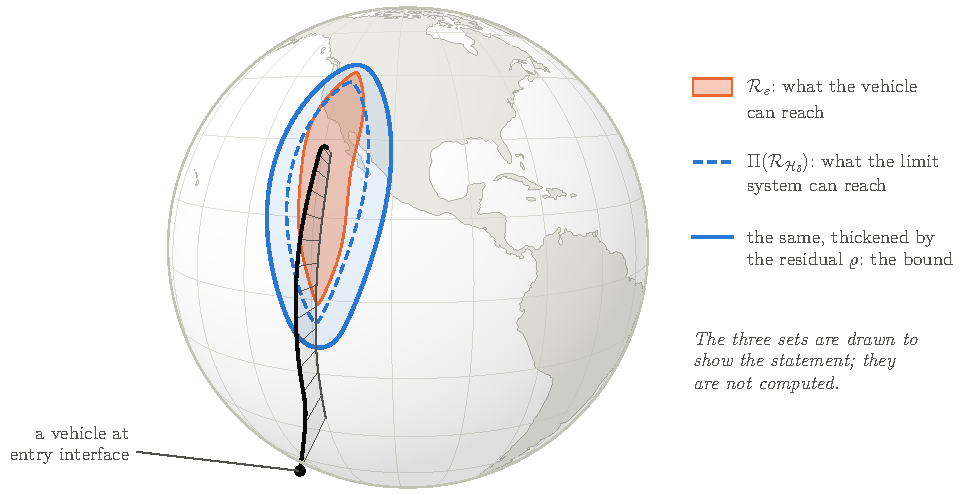
\includegraphics[width=6.5in]{figures/reachable-set.pdf}
  \caption{The statement aimed at, drawn on the ground. The trajectory is an
    example, a lunar-return skip entry simulated from a published entry
    state~\cite{rea2024orion}, with altitude drawn twelve times too large
    and a post each minute. The three sets are an illustration and are not
    computed: what the vehicle can reach, what the limit system can reach,
    and the second thickened by a margin, which is the bound. The first may
    leave the second, but by no more than the margin.}
\end{figure}

\head{The gap.}
One outer bound is free, and it shows what is missing. Drag dissipates
energy at the rate $P = DV$ per unit mass, so a path of length~$R$ costs at
least $R\,D_{\min}$, and with $\Delta\mathcal{E}$ the energy there is to
lose, $R\le\Delta\mathcal{E}/D_{\min}$. It holds for every control because
it uses nothing about the control, and it is useless for the same reason:
it charges the whole flight at the thinnest air the corridor allows, so that
across a skip it says nothing. The tools that use more do not reach the
question. A Hamilton--Jacobi equation on a grid stops near five
states~\cite{bansal2017hamilton}, and a rigid body has thirteen; a
flowpipe~\cite{chen2013flowstar} encloses one vehicle, one initial set and
one horizon, and tends to widen along weakly damped motion; and guidance is
validated by sampling~\cite{lu2014entry}.

\head{What the free bound ignores.}
It ignores \emph{when} the energy is lost. The ratio of the atmosphere's
scale height to the planet's radius, $\eps = H_s/R_e\approx 10^{-3}$, is a
small parameter, and as it vanishes a trajectory comes apart into three
motions. Above the atmosphere it follows an arc under
gravity and loses nothing. On the equilibrium glide, where lift balances
weight less centrifugal relief, it loses energy slowly. And in a
\emph{pass} it dips into dense air, turns, and sheds a fixed share of its
energy in a vanishing time. A pass is also where a control decides where
the vehicle goes, and it is what the standard relaxation loses. In the space
of occupation measures the dynamics are a linear constraint and an outer
bound is certified by a dual pair of functions~\cite{henrion2014convex}; but
an occupation measure weighs each interval of time by its length, and in the
limit a pass has none.

The proposal is to keep the account in energy instead. Along every
trajectory, for every control and every selection of an interval-enclosed
vector field, the energy in the rotating frame satisfies
$\dot{\mathcal{E}} = -P\le 0$, so the dissipation has total mass at most
$\Delta\mathcal{E}$, uniformly in~$\eps$. On the rescaled time
$\tau = t/\sqrt{\eps}$ its normalized density is a sequence of probability
densities on the line, and Lions' concentration-compactness
lemma~\cite{lions1984concentration1} applies as stated; the reading to be
argued is that vanishing is the glide, compactness a pass, and dichotomy
passes that separate. Along a subsequence the dissipation converges to a
measure $p\dd t + \sum_j a_j\delta_{t_j} + \pi_c$, with at most
$\Delta\mathcal{E}/\delta$ atoms above~$\delta$. What has to be proved first
is what the atoms carry: that the velocity converges to a function of
bounded variation that jumps only at them, and that the limit of a
trajectory satisfies a Liouville equation with a jump term they carry.

\head{The theorem aimed at.}
The atoms are to be the passes, and the limit a hybrid system
$\mathcal{H}_\delta$ in a few slow coordinates. It \emph{flows} along
gravity arcs and along the glide, and it \emph{jumps}, at most
$K_\delta\le\Delta\mathcal{E}/\delta$ times, through a set-valued
\emph{pass map}: skeleton and bubbles, in the language of profile
decompositions~\cite{bahouri1999high}. The statement aimed at is one at
fixed~$\eps$, uniform over the admissible family:
\[
  \calR_\eps(T) \;\subseteq\; \Pi\bigl(\calR_{\mathcal{H}_\delta}(T)\bigr)
  \;\oplus\; \B\bigl(\varrho(\eps,\delta)\bigr),
\]
the reachable set of the full system inside that of the limit system, read
back in the full coordinates and thickened by a ball of explicit radius, as
the figure draws it. Compactness gives structure and no constants; in
the wave-equation theory the analogous uniform bound is obtained by
contradiction, with a constant its authors say they cannot
describe~\cite{bahouri1999high}. Here the constants are to come from direct
estimates, in closed form in the corridor bounds and the interval widths.

\head{The obstacle.}
With $z$ the altitude above the glide in scale heights and $G = g - V^2/r$
the acceleration that lift balances, the vertical motion is, to leading
order,
\[
  \ddot z \;=\; \frac{G}{H_s}\,\bigl(c(t)\,e^{-z} - 1\bigr),
  \qquad
  \frac{\mathrm{d}}{\mathrm{d}t}\Bigl[\tfrac12\dot z^2
     + \tfrac{G}{H_s}\bigl(e^{-z}+z\bigr)\Bigr]
  \;=\; \tfrac{G}{H_s}\,(c-1)\,e^{-z}\,\dot z ,
\]
where $c(t)$ is the control, the vertical lift against a reference. The
glide is the equilibrium, the phugoid its small oscillation, and a skip its
large one. The frequency grows like $\eps^{-1/2}$ and the damping rate does
not depend on $\eps$, so the damping ratio is $O(\sqrt{\eps})$: the glide
is not a normally hyperbolic slow manifold~\cite{fenichel1979geometric},
and no boundary-layer estimate brings a trajectory onto it. And the control
pumps or damps the oscillation at will, by the identity on the right. The
amplitude is therefore a slow, controlled coordinate of the limit system,
and what is needed is an averaging theorem \emph{with constants}, uniform
over a set-valued field, and valid for \emph{every} trajectory, including
those that pass through resonance: the attitude frequency grows with the
square root of the dynamic pressure and sweeps through the others on every
pass. The available results give orders, not bounds, and through a
resonance they hold outside a set of small
measure~\cite{sanders2007averaging}, which an outer bound cannot discard.
This is the critical path, and it is the part of the program for which I
am looking for an advisor.

\head{What is open.}
All of it: this is a proposal, and it claims no result. Three statements
carry it. The limit: that the jump term is carried on the graph of the pass
map, and that no singular continuous part survives. Composition: a
factorization through pass maps and flows with an explicit matching
remainder, uniform over the interval field, where the classical matched
expansions treat one trajectory~\cite{shi1971skip}. And averaging through
resonance, with constants, which is the critical path and is to be attacked
first.

\printbibliography[heading=none]

\end{document}
